\documentclass[a4paper,14pt]{extreport} % формат документа

\usepackage{amsmath}
\usepackage{cmap} % поиск в ПДФ
\usepackage[T2A]{fontenc} % кодировка
\usepackage[utf8]{inputenc} % кодировка исходного текста
\usepackage[english,russian]{babel} % локализация и переносы
\usepackage[left = 2cm, right = 1cm, top = 2cm, bottom = 2 cm]{geometry} % поля
\usepackage{listings}
\usepackage{graphicx} % для вставки рисунков
\usepackage{amsmath}
\usepackage{float}
\usepackage{multirow}
\graphicspath{{pictures/}}
\DeclareGraphicsExtensions{.pdf,.png,.jpg}
\newcommand{\anonsection}[1]{\section*{#1}\addcontentsline{toc}{section}{#1}}

\lstset{ %
	language=python,                % Язык программирования 
	numbers=left,                   % С какой стороны нумеровать          
	frame=single,                    % Добавить рамку
	escapebegin=\begin{russian}\commentfont,
    escapeend=\end{russian},
    literate={Ö}{{\"O}}1
    {Ä}{{\"A}}1
    {Ü}{{\"U}}1
    {ß}{{\ss}}1
    {ü}{{\"u}}1
    {ä}{{\"a}}1
    {ö}{{\"o}}1
    {~}{{\textasciitilde}}1
    {а}{{\selectfont\char224}}1
    {б}{{\selectfont\char225}}1
    {в}{{\selectfont\char226}}1
    {г}{{\selectfont\char227}}1
    {д}{{\selectfont\char228}}1
    {е}{{\selectfont\char229}}1
    {ё}{{\"e}}1
    {ж}{{\selectfont\char230}}1
    {з}{{\selectfont\char231}}1
    {и}{{\selectfont\char232}}1
    {й}{{\selectfont\char233}}1
    {к}{{\selectfont\char234}}1
    {л}{{\selectfont\char235}}1
    {м}{{\selectfont\char236}}1
    {н}{{\selectfont\char237}}1
    {о}{{\selectfont\char238}}1
    {п}{{\selectfont\char239}}1
    {р}{{\selectfont\char240}}1
    {с}{{\selectfont\char241}}1
    {т}{{\selectfont\char242}}1
    {у}{{\selectfont\char243}}1
    {ф}{{\selectfont\char244}}1
    {х}{{\selectfont\char245}}1
    {ц}{{\selectfont\char246}}1
    {ч}{{\selectfont\char247}}1
    {ш}{{\selectfont\char248}}1
    {щ}{{\selectfont\char249}}1
    {ъ}{{\selectfont\char250}}1
    {ы}{{\selectfont\char251}}1
    {ь}{{\selectfont\char252}}1
    {э}{{\selectfont\char253}}1
    {ю}{{\selectfont\char254}}1
    {я}{{\selectfont\char255}}1
    {А}{{\selectfont\char192}}1
    {Б}{{\selectfont\char193}}1
    {В}{{\selectfont\char194}}1
    {Г}{{\selectfont\char195}}1
    {Д}{{\selectfont\char196}}1
    {Е}{{\selectfont\char197}}1
    {Ё}{{\"E}}1
    {Ж}{{\selectfont\char198}}1
    {З}{{\selectfont\char199}}1
    {И}{{\selectfont\char200}}1
    {Й}{{\selectfont\char201}}1
    {К}{{\selectfont\char202}}1
    {Л}{{\selectfont\char203}}1
    {М}{{\selectfont\char204}}1
    {Н}{{\selectfont\char205}}1
    {О}{{\selectfont\char206}}1
    {П}{{\selectfont\char207}}1
    {Р}{{\selectfont\char208}}1
    {С}{{\selectfont\char209}}1
    {Т}{{\selectfont\char210}}1
    {У}{{\selectfont\char211}}1
    {Ф}{{\selectfont\char212}}1
    {Х}{{\selectfont\char213}}1
    {Ц}{{\selectfont\char214}}1
    {Ч}{{\selectfont\char215}}1
    {Ш}{{\selectfont\char216}}1
    {Щ}{{\selectfont\char217}}1
    {Ъ}{{\selectfont\char218}}1
    {Ы}{{\selectfont\char219}}1
    {Ь}{{\selectfont\char220}}1
    {Э}{{\selectfont\char221}}1
    {Ю}{{\selectfont\char222}}1
    {Я}{{\selectfont\char223}}1
    {і}{{\selectfont\char105}}1
    {ї}{{\selectfont\char168}}1
    {є}{{\selectfont\char185}}1
    {ґ}{{\selectfont\char160}}1
    {І}{{\selectfont\char73}}1
    {Ї}{{\selectfont\char136}}1
    {Є}{{\selectfont\char153}}1
    {Ґ}{{\selectfont\char128}}1
}

\begin{document}
\begin{titlepage}

    \begin{table}[H]
        \centering
        \footnotesize
        \begin{tabular}{cc}
            \multirow{8}{*}{
\includegraphics[scale=0.35]{bmstu.jpg}}
            & \\
            & \\
            & \textbf{Министерство науки и высшего образования Российской Федерации} \\
            & \textbf{Федеральное государственное бюджетное образовательное учреждение} \\
            & \textbf{высшего образования} \\
            & \textbf{<<Московский государственный технический} \\
            & \textbf{университет имени Н.Э. Баумана>>} \\
            & \textbf{(МГТУ им. Н.Э. Баумана)} \\
        \end{tabular}
    \end{table}

    \vspace{-2.5cm}

    \begin{flushleft}
        \rule[-1cm]{\textwidth}{3pt}
        \rule{\textwidth}{1pt}
    \end{flushleft}

    \begin{flushleft}
        \small
        ФАКУЛЬТЕТ
        \underline{<<Информатика и системы управления>>\ \ \ \ \ \ \ 
        \ \ \ \ \ \ \ \ \ \ \ \ \ \ \ \ \ \ \ \ \ \ \ \ \ \ \ \ \ \ \ 
    \ \ \ \ \ \ \ \ \ \ \ \ \ \ \ } \\
        КАФЕДРА
        \underline{<<Программное обеспечение ЭВМ и
        информационные технологии>>
        \ \ \ \ \ \ \ \ \ \ \ \ \ \ \ \ \ \ \ \ }
    \end{flushleft}

    \vspace{2cm}

    \begin{center}
        \textbf{Лабораторная работа № 4} \\
        \vspace{0.5cm}
    \end{center}

    \vspace{4cm}

    \begin{flushleft}
        \begin{tabular}{ll}
            \textbf{Дисциплина} & Моделирование.  \\
            \textbf{Тема} & Программно-алгоритмическая реализация моделей на основе \\
            & дифференциальных уравнений в частных производных \\
            & с краевыми условиями II и  III рода.\\
            \\
            \textbf{Студент} & Сиденко А.Г. \\
            \textbf{Группа} & ИУ7-63Б \\
            \textbf{Оценка (баллы)} & \\
            \textbf{Преподаватель} & Градов В.М.   \\
        \end{tabular}
    \end{flushleft}

    \vspace{4cm}

   \begin{center}
        Москва, 2020 г.
    \end{center}

\end{titlepage}

\textbf{Цель работы:} Получение навыков разработки  алгоритмов решения смешанной краевой задачи при реализации моделей, построенных на квазилинейном уравнении параболического типа. 

\begin{enumerate}
\item Дано:
$$k(T)=a_1(b_1+c_1T^{m_1})$$
$$c(T)=a_2+b_2T^{m_2}-\frac{c_2}{T^2}$$
$$a_1=0.0134$$
$$b_1=1$$
$$c_1=4.35\cdot10^{-4}$$
$$m_1=1$$
$$a_2=2.049$$
$$b_2=0.563\cdot10^{-3}$$
$$c_2=0.528\cdot10^{5}$$
$$m_2=1$$
$$\alpha(x)=\frac{c}{x-d}$$
$$\alpha_0=0.05$$
$$\alpha_N=0.01$$
$$l=10$$
$$T_0=300$$
$$R=0.5$$
$$F(t)=50$$

\item Уравнение

\begin{equation}
c(T)\frac{\partial T}{\partial t}=\frac{\partial}{\partial x}\bigg(k(T)\frac{\partial T}{\partial x}\bigg)-\frac{2}{R}\alpha(x)T+\frac{2T_0}{R}\alpha(x)
\end{equation}

\item Краевые условия

$$
 \begin{cases}
 t=0, ~T(x,0)=T_0
   \\
   x=0, ~-k(T(0))\frac{\partial T}{\partial x}=F_0
   \\
   x =l,~-k(l)\frac{\partial T}{\partial x}=\alpha_N(T(l)-T_0)
 \end{cases}
$$

Функция $\alpha(x)$ задана:

$$\alpha(x)=\frac{c}{x-d}$$, где 

$$c=-\alpha_0d=\frac{\alpha_0\alpha_Nl}{\alpha_0-\alpha_N}, d = \frac{\alpha_Nl}{\alpha_N-\alpha_0}$$

\item Разностная схема

\begin{equation}
\begin{aligned}
&\buildrel\,\,\frown\over{A}_n\buildrel\,\,\frown\over{y}_{n-1}-\buildrel\,\,\frown\over{B}_n\buildrel\,\,\frown\over{y}_n+\buildrel\,\,\frown\over{D}_n\buildrel\,\,\frown\over{y}_{n+1}=-\buildrel\,\,\frown\over{F}_n, 1\le n\le N-1\\
&\buildrel\,\,\frown\over{A}_n=\buildrel\,\,\frown\over{\chi}_{n-\frac{1}{2}}\frac{\tau}{h},\\
&\buildrel\,\,\frown\over{B}_n=\buildrel\,\,\frown\over{A}_n+\buildrel\,\,\frown\over{D}_n+\buildrel\,\,\frown\over{c}_nh+p_nh\tau,\\
& \buildrel\,\,\frown\over{D}_n=\buildrel\,\,\frown\over{\chi}_{n+\frac{1}{2}}\frac{\tau}{h}, \\
&\buildrel\,\,\frown\over{F}_n=f_nh\tau+\buildrel\,\,\frown\over{c}_ny_nh\\
\end{aligned}
\end{equation}

\item Краевые условия

Обозначим:

\begin{equation}
\begin{aligned}
&F=-k(T)\frac{\partial T}{\partial x}\\
&p(x)=\frac{2}{R}\alpha(x)\\
&f(x)=\frac{2T_0}{R}\alpha(x)\\
\end{aligned}
\end{equation}

Разностные аналоги краевых условий при x=0:

\begin{multline}
\bigg(\frac{h}{8}\buildrel\,\,\frown\over{c}_{\frac{1}{2}}+ \frac{h}{4}\buildrel\,\,\frown\over{c}_0+\buildrel\,\,\frown\over{\chi}_{\frac{1}{2}}\frac{\tau}{h}+\frac{\tau h}{8}p_{\frac{1}{2}}+\frac{\tau h}{4}p_0\bigg)\buildrel\,\,\frown\over{y}_0+\bigg(\frac{h}{8}\buildrel\,\,\frown\over{c}_{\frac{1}{2}}-\buildrel\,\,\frown\over{\chi}_{\frac{1}{2}}\frac{\tau}{h}+\frac{\tau h}{8}p_{\frac{1}{2}}\bigg)\buildrel\,\,\frown\over{y}_1=\\
= \frac{h}{8}\buildrel\,\,\frown\over{c}_{\frac{1}{2}}(y_0+y_1)+\frac{h}{4}\buildrel\,\,\frown\over{c}_0y_0+\buildrel\,\,\frown\over{F}\tau+\frac{\tau h}{4}(\buildrel\,\,\frown\over{f}_{\frac{1}{2}}+\buildrel\,\,\frown\over{c}_0)
\end{multline}

Взято из лекции. 

Разностные аналоги краевых условий при x=l, вывод:

Проинтегрируем уравнение 1 с учетом замен 3 на отрезке $[x_{N-\frac{1}{2}},x_N]$

\begin{multline*}
\int^{x_N}_{x_{N-{\frac{1}{2}}}}dx=-\int^{t_{m+1}}_{t_{m}}dt\int^{x_N}_{x_{N-{\frac{1}{2}}}}\frac{\partial F}{\partial x}dx-\int^{x_N}_{x_{N-{\frac{1}{2}}}}dx\int^{t_{m+1}}_{t_{m}}p(x)Tdt+\\
+\int^{x_N}_{x_{N-{\frac{1}{2}}}}dx\int^{t_{m+1}}_{t_{m}}f(T)dt
\end{multline*}

Вычисляем интегралы методом правых прямоугольников. 

\begin{multline*}
\int^{x_N}_{x_{N-{\frac{1}{2}}}}\buildrel\,\,\frown\over{c}(\buildrel\,\,\frown\over{T}-T)dx=-\int^{t_{m+1}}_{t_{m}}(F_N-F_{N-\frac{1}{2}})dt-\int^{x_N}_{x_{N-{\frac{1}{2}}}}p\buildrel\,\,\frown\over{T}\tau dx+\int^{x_N}_{x_{N-{\frac{1}{2}}}}\buildrel\,\,\frown\over{f}\tau dx
\end{multline*}

Вычисляем интегралы методом трапеций, а первый справа -- методом правых прямоугольников. 

\begin{multline*}
\big(\buildrel\,\,\frown\over{c}_{N}(\buildrel\,\,\frown\over{y}_N-y_N)+\buildrel\,\,\frown\over{c}_{N-\frac{1}{2}}(\buildrel\,\,\frown\over{y}_{N-\frac{1}{2}}-y_{N-\frac{1}{2}})\big)\frac{h}{4}=-\tau(\buildrel\,\,\frown\over{F}_N-\buildrel\,\,\frown\over{F}_{N-\frac{1}{2}})-\\
-\big(p_N\buildrel\,\,\frown\over{y}_N+p_{N-\frac{1}{2}}\buildrel\,\,\frown\over{y}_{N-\frac{1}{2}}\big)\tau\frac{h}{4} +(\buildrel\,\,\frown\over{f}_N+\buildrel\,\,\frown\over{f}_{N-\frac{1}{2}})\tau \frac{h}{4}
\end{multline*}

Зная

\begin{equation}
\begin{aligned}
&\buildrel\,\,\frown\over{F}_N=\alpha_N(\buildrel\,\,\frown\over{y}_N-T_0)\\
&\buildrel\,\,\frown\over{F}_{N-\frac{1}{2}}=\buildrel\,\,\frown\over{\chi}_{N-\frac{1}{2}}\frac{\buildrel\,\,\frown\over{y}_{N-1}-\buildrel\,\,\frown\over{y}_N}{h}\\
\end{aligned}
\end{equation}

\begin{multline*}
\buildrel\,\,\frown\over{c}_{N}\buildrel\,\,\frown\over{y}_N\frac{h}{4}-\buildrel\,\,\frown\over{c}_{N}y_N\frac{h}{4}+\buildrel\,\,\frown\over{c}_{N-\frac{1}{2}}\buildrel\,\,\frown\over{y}_{N}\frac{h}{8}+\buildrel\,\,\frown\over{c}_{N-\frac{1}{2}}\buildrel\,\,\frown\over{y}_{N-1}\frac{h}{8}-\buildrel\,\,\frown\over{c}_{N-\frac{1}{2}}{y}_{N}\frac{h}{8}-\\
-\buildrel\,\,\frown\over{c}_{N-\frac{1}{2}}{y}_{N-1}\frac{h}{8}=-\tau\alpha_N\buildrel\,\,\frown\over{y}_N+\tau\alpha_NT_0+\tau\buildrel\,\,\frown\over{\chi}_{N-\frac{1}{2}}\frac{\buildrel\,\,\frown\over{y}_{N-1}}{h}-\tau\buildrel\,\,\frown\over{\chi}_{N-\frac{1}{2}}\frac{\buildrel\,\,\frown\over{y}_{N}}{h}-\\
-p_N\buildrel\,\,\frown\over{y}_N\tau\frac{h}{4}-p_{N-\frac{1}{2}}\buildrel\,\,\frown\over{y}_{N}\tau\frac{h}{8}-p_{N-\frac{1}{2}}\buildrel\,\,\frown\over{y}_{N-1}\tau\frac{h}{8}  +(\buildrel\,\,\frown\over{f}_N+\buildrel\,\,\frown\over{f}_{N-\frac{1}{2}})\tau \frac{h}{4}
\end{multline*}

\begin{multline}
\buildrel\,\,\frown\over{y}_{N-1}\bigg(\buildrel\,\,\frown\over{c}_{N-\frac{1}{2}}\frac{h}{8}  - \frac{\tau\buildrel\,\,\frown\over{\chi}_{N-\frac{1}{2}}}{h} + p_{N-\frac{1}{2}}\tau\frac{h}{8}  \bigg)+\\
+ \buildrel\,\,\frown\over{y}_N\bigg( \buildrel\,\,\frown\over{c}_{N}\frac{h}{4} + \buildrel\,\,\frown\over{c}_{N-\frac{1}{2}}\frac{h}{8} + \tau\alpha_N +\frac{ \tau\buildrel\,\,\frown\over{\chi}_{N-\frac{1}{2}}}{h} +p_N\tau\frac{h}{4}+p_{N-\frac{1}{2}}\tau\frac{h}{8} \bigg)=\\
=\buildrel\,\,\frown\over{c}_{N-\frac{1}{2}}\bigg({y}_{N}\frac{h}{8}+{y}_{N-1}\frac{h}{8} \bigg) + \buildrel\,\,\frown\over{c}_{N}y_N\frac{h}{4}+\tau\alpha_NT_0+(\buildrel\,\,\frown\over{f}_N+\buildrel\,\,\frown\over{f}_{N-\frac{1}{2}})\tau \frac{h}{4}
\end{multline}

Соответственно из этих краевых условий (формулы 4, 6) можем найти коэффициенты $K_0,~K_N,~M_0,~M_N,~P_0,~P_N$. 

\begin{equation}
\begin{cases}
\buildrel\,\,\frown\over{K}_0\buildrel\,\,\frown\over{y}_0+\buildrel\,\,\frown\over{M}_0\buildrel\,\,\frown\over{y}_1=\buildrel\,\,\frown\over{P}_0\\
\buildrel\,\,\frown\over{A}_n\buildrel\,\,\frown\over{y}_{n-1}-\buildrel\,\,\frown\over{B}_n\buildrel\,\,\frown\over{y}_n+\buildrel\,\,\frown\over{D}_n\buildrel\,\,\frown\over{y}_{n+1}=-\buildrel\,\,\frown\over{F}_n, 1\le n\le N-1\\
\buildrel\,\,\frown\over{K}_N\buildrel\,\,\frown\over{y}_N+\buildrel\,\,\frown\over{M}_{N-1}\buildrel\,\,\frown\over{y}_{N-1}=\buildrel\,\,\frown\over{P}_N\\
\end{cases}
\end{equation}

Система 7 решается методом простых итераций. 

\item Метод простых итераций

Обозначим текущую итерацию s, а предыдущую (s-1) , тогда итерационный процесс организуется по схеме

\begin{equation}
{A}_n^{s-1}{y}_{n+1}^{s}-{B}_n^{s-1}{y}_n^{s}+{D}^{s-1}_n{y}_{n-1}^{s}=-{F}^{s-1}_n
\end{equation}

Решение которой осуществляется методом прогонки. Итерации прекращаются при условии

\begin{equation*}
\max\bigg|\frac{y^s_n-y^{s-1}_n}{y^s_n}\bigg|\le\varepsilon, \text{для всех } n=\overline{0 ... N}
\end{equation*}

\end{enumerate}

\textbf{Приведем листинг. }

\begin{lstlisting}[caption=Заданные параметры]
a1 = 0.0134
b1 = 1
c1 = 4.35e-4
m1 = 1
a2 = 2.049
b2 = 0.563e-3
c2 = 0.528e5
m2 = 1
alpha0 = 0.05
alphaN = 0.01
l = 10
T0 = 300
R = 0.5
F0 = 50
h = 0.01
t = 1
\end{lstlisting}

\begin{lstlisting}[caption=Коэффициенты теплопроводности материала стержня и теплоотдачи при обдуве; теплоемкость]
def k(T):
    return a1 * (b1 + c1 * T ** m1)

def c(T):
    return a2 + b2 * T ** m2 - c2 / T ** 2

def alpha(x):
    d = (alphaN * l) / (alphaN - alpha0)
    c = - alpha0 * d
    return c / (x - d)
\end{lstlisting}

\begin{lstlisting}[caption=Выполненные замены]
def p(x):
    return 2 * alpha(x) / R

def f(x):
    return 2 * alpha(x) * T0 / R
\end{lstlisting}

\begin{lstlisting}[caption=Метод средних для вычисления значения функций]
def func_plus_1_2(x, step, func):
    return (func(x) + func(x + step)) / 2

def func_minus_1_2(x, step, func):
    return (func(x) + func(x - step)) / 2
\end{lstlisting}

\begin{lstlisting}[caption=Функции для нахождения параметров разностной схемы]
def A(T):
    return func_minus_1_2(T, t, k) * t / h

def D(T):
    return func_plus_1_2(T, t, k) * t / h

def B(x, T):
    return A(T) + D(T) + c(T) * h + p(x) * h * t

def F(x, T):
    return f(x) * h * t + c(T) * T * h
\end{lstlisting}

\begin{lstlisting}[caption=Метод прогонки]
def run_through(prevT):
    K0 = h / 8 * func_plus_1_2(prevT[0], t, c) + \
                   h / 4 * c(prevT[0]) + \
                   func_plus_1_2(prevT[0], t, k) * t / h + \
                   t * h / 8 * p(h / 2) + t * h / 4 * p(0)

    M0 = h / 8 * func_plus_1_2(prevT[0], t, c) - \
                   func_plus_1_2(prevT[0], t, k) * t / h + \
                   t * h * p(h / 2) / 8

    P0 = h / 8 * func_plus_1_2(prevT[0], t, c) * (prevT[0]+ \
                   prevT[1]) + \
                   h / 4 * c(prevT[0]) * prevT[0] + \
                   F0 * t + t * h / 8 * (3 * f(0) + f(h))

    KN = h / 8 * func_minus_1_2(prevT[-1], t, c) + \
                   h / 4 * c(prevT[-1]) + \
                   func_minus_1_2(prevT[-1], t, k) * t / h + \
                   t * alphaN + \
                   t * h / 8 * p(l - h / 2) + t * h / 4 * p(l)

    MN = h / 8 * func_minus_1_2(prevT[-1], t, c) - \
                   func_minus_1_2(prevT[-1], t, k) * t / h + \
                   t * h * p(l - h / 2) / 8

    PN = h / 8 * func_minus_1_2(prevT[-1], t, c) * \
                   (prevT[-1] + prevT[-2]) + \
                   h / 4 * c(prevT[-1]) * prevT[-1] + \
                   t * alphaN * T0 + \
                   t * h / 4 * (f(l) + f(l - h / 2))

    # Прямой ход
    eps = [0, -M0 / K0]
    eta = [0, P0 / K0]

    x = h
    n = 1
    while (x + h < l):
        eps.append(D(prevT[n]) / (B(x, prevT[n]) - \
                   A(prevT[n]) * eps[n]))
        eta.append((F(x, prevT[n]) + \
                   A(prevT[n]) * eta[n]) / (B(x, prevT[n]) \
                   - A(prevT[n]) * eps[n]))
        n += 1
        x += h

    # Обратный ход
    y = [0] * (n + 1)
    y[n] = (PN - MN * eta[n]) / (KN + MN * eps[n])

    for i in range(n - 1, -1, -1):
        y[i] = eps[i + 1] * y[i + 1] + eta[i + 1]

    return y
\end{lstlisting}

\begin{lstlisting}[caption=Метод простых итераций]
def check_eps(T, newT):
    for i, j in zip(T, newT):
        if fabs((i - j) / j) > 1e-3:
            return True
    return False

def check_iter(T, newT):
    max = fabs((T[0] - newT[0]) / newT[0])
    for i, j in zip(T, newT):
        d = fabs(i - j) / j
        if d > max:
            max = d
    return max < 1e-2

def iter_method():
    result = []
    n = int(l / h)
    T = [T0] * (n + 1)
    newT = [0] * n
    
    result.append(T)

    while (True):
        buf = T
        while True:
            newT = run_through(buf)
            if check_iter(buf, newT):
                break
            buf = newT

        result.append(newT)
        if (check_eps(T, newT) == False):
            break

        T = newT

    return result
\end{lstlisting}
\newpage 
\textbf{Результаты работы программы. }

\begin{enumerate}
\item График зависимости температуры от координаты при нескольких фиксированных значениях времени.

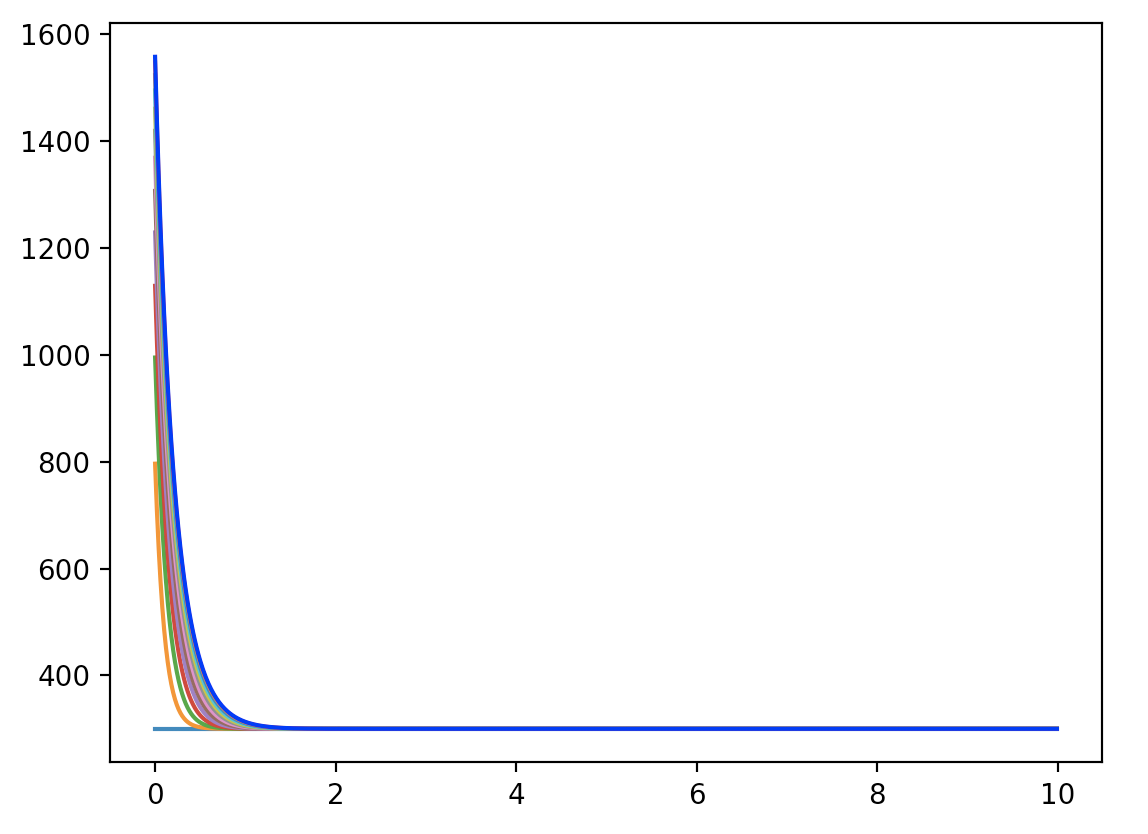
\includegraphics[scale=0.85]{1}

На рисунке представлены графики зависимости температуры от координаты при фиксированных t = 0, 2, 4, .... 

Последняя -- синяя кривая соответствует установившемуся режиму, когда поле перестает меняться с точностью 1е-3. 

\item График зависимости температуры от времени при нескольких фиксированных значениях координаты. 

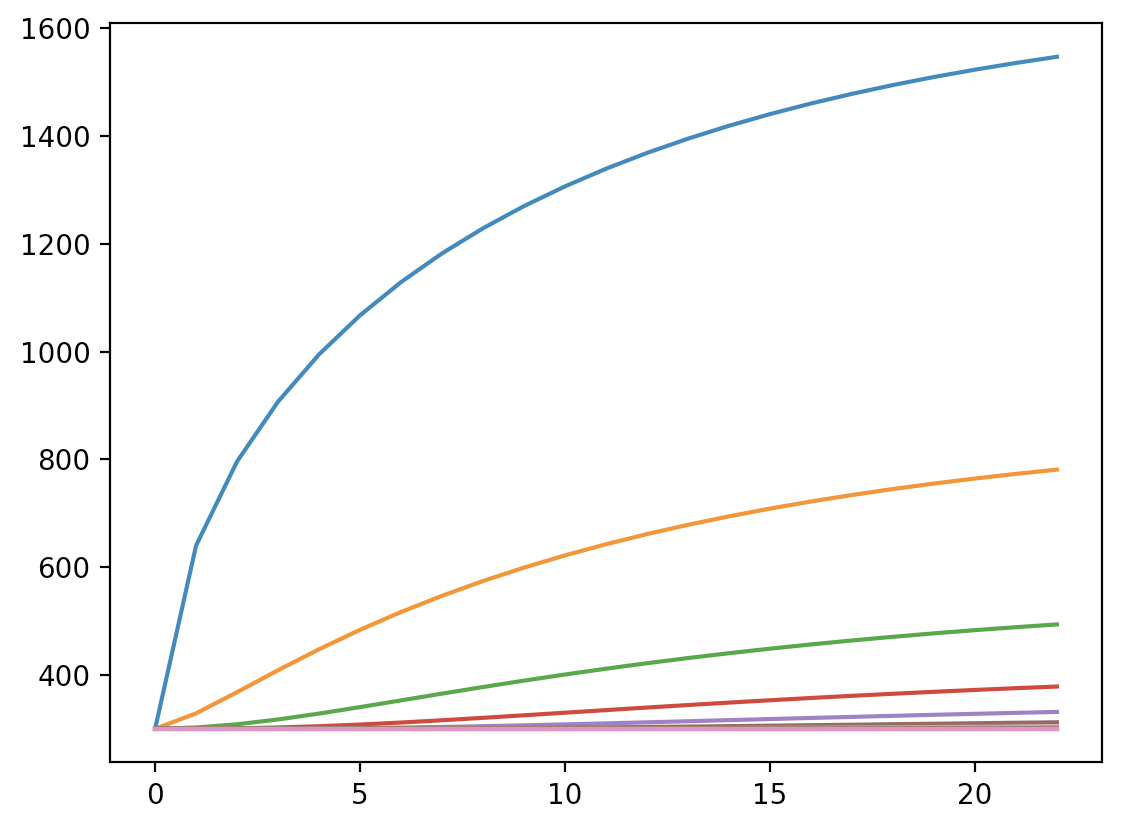
\includegraphics[scale=0.85]{2}

На рисунке представлены графики зависимости температуры от времени при фиксированных x = 0, 0.2, 0.4, .. 3.2

\end{enumerate}

\newpage
\textbf{Ответы на вопросы. }

\begin{enumerate}
\item Тестирование

\begin{enumerate}
\item Свойства материала стержня привязаны к температуре, теплоемкость и коэффициент теплопроводности  зависят от T, поменяем зависимости установим зависимости T от х, а с = 0. Тогда температурное поле T(x,t) должно совпасть с температурным распределением T(x) из лабораторной 3. 

\begin{figure}[ht]\center
	\begin{tabular}{cc}
		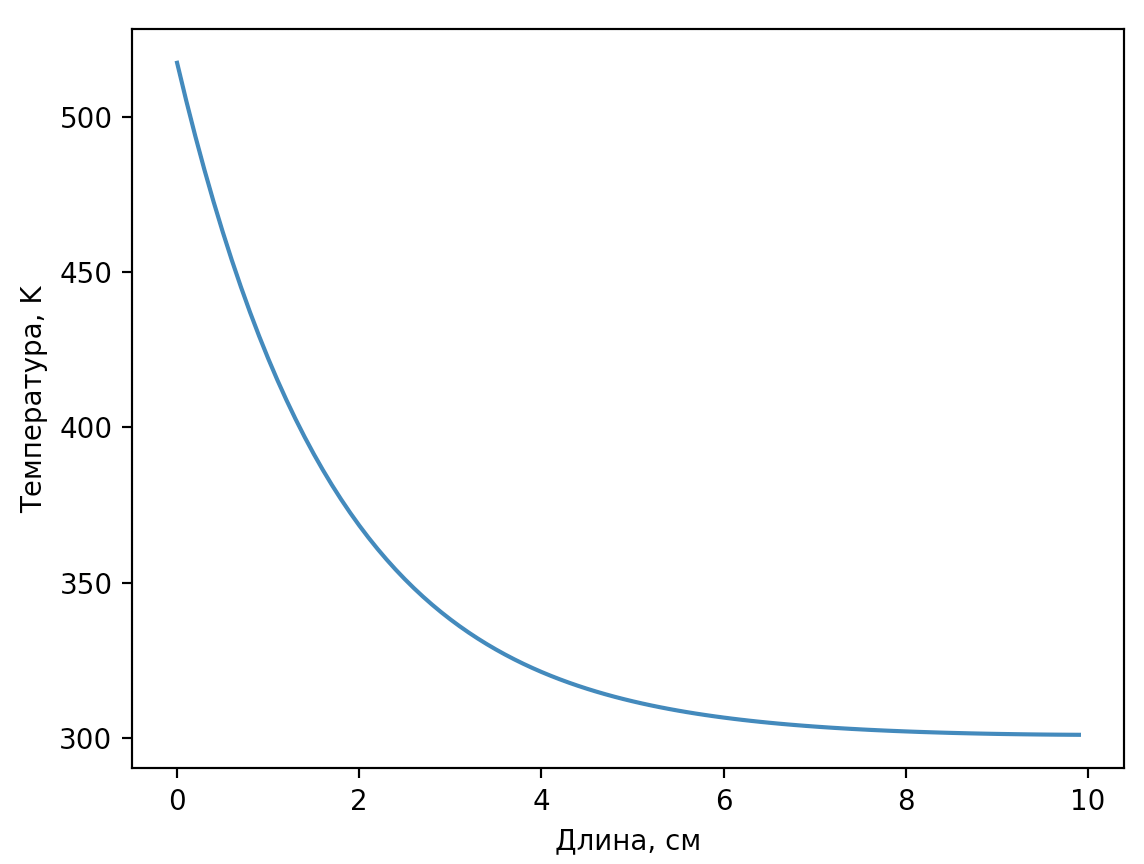
\includegraphics[width=90mm]{3} & 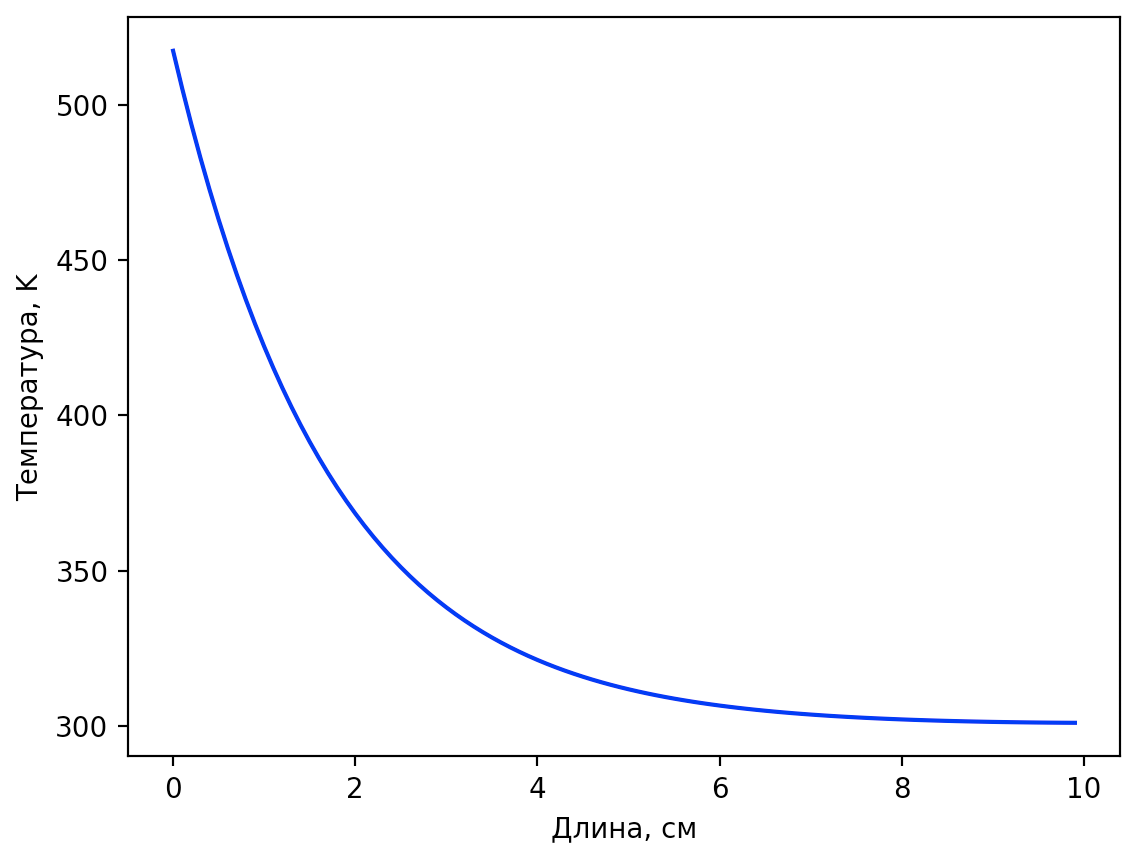
\includegraphics[width=90mm]{4}
	\end{tabular}
	\\ На левом рисунке представлен график из 3 работы, а на правом из текущей с измененными параметрами. 
\end{figure}
  
\item Если после разогрева стержня положить поток = 0, то будет происходить остывание, пока температура не выровняется по всей длине и не станет равной To.

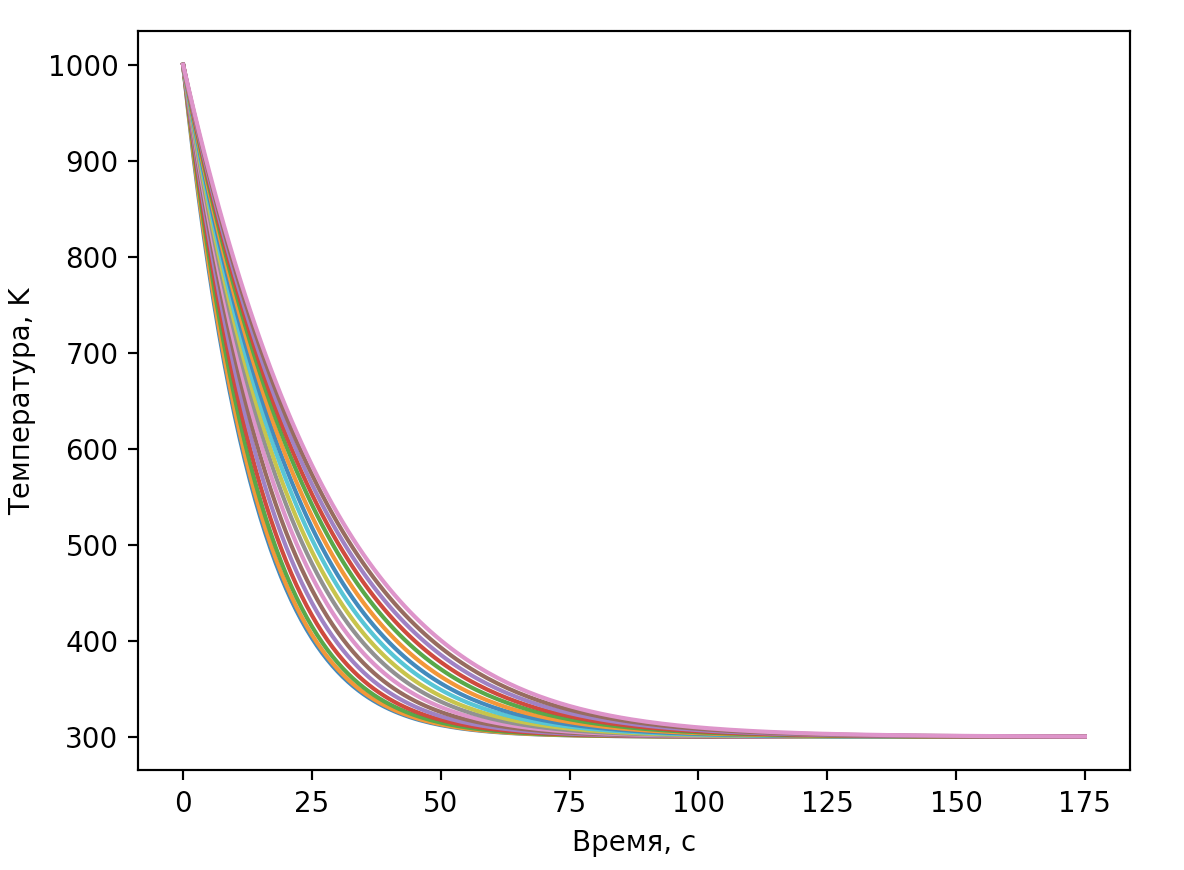
\includegraphics[scale=0.8]{5}

Нагреем весь стержень до температуры 1000К, поток установим в 0, температура окружающей среды оставим 300К. 

На данном рисунке при фиксированных x = 0, 0.2, 0.4, .. 3.2 представлены графики зависимости температуры от времени. 

\end{enumerate}

\item Выполните, полагая для простоты, что все коэффициенты зависят только от одной переменной $y_n$. Приведите линеаризованный вариант уравнения и опишите алгоритм его решения.


\end{enumerate}

\end{document}